\section{Lustre Generic Filesystem Wraper Layer: fsfilt}

Lustre provides a generic wrapper layer named~\emph{fsfilt} to interface
between the underlying local filesystem and Lustre. The upper
layer,~\url{obd_filter}, uses generic functions provided by the~\url{fsfilt}
layer, and then~\url{fsfilt} layer passes these calls into a filesystem specific
implementation. These specific implementations are interfaces to the particular
underlying filesystem. The fsfilt calls the local filesystem by using tiny
wrappers targeted for the particular filesystem (e.g.,~\url{fsfilt_ext3}
for~\emph{ext3} filesystem and~\url{fsfilt_reiserfs} for~\emph{Reiserfs3}
filesystem). This section outlines details of the~\url{fsfilt} layer and
analyzes~\url{fsfilt_ext3} as an example interface implementation.

\subsection{Overview}
\label{sec:fsfilt_linux}

The ~\url{fsfilt} framework is largely defined by
the~\url{lustre/include/luste_fsfilt.h} file. In this file~\url{struct
fsfilt_operations} defines operations required from the underlying filesystem.
At the~\url{obd_filter} registration time, the system tells what filesystem it is
built under and Lustre calls the required filesystem registration operations.
This is done during the kernel module (e.g.,~\url{ldiskfs},~\url{fsfilt_ext3})
initialization phase. Corresponding source code for each filesystem
implementation is located in~\url{lustre/lvfs}.  However,
the~\url{fsfilt_ldfiskfs.c} file will be missing with the~\emph{HEAD CVS}
checkout, because it is generated at build time from~\url{ldiskfs_ext3.c} (same
as in other CVS branches) by taking~\url{fsfilt_ext3.c} and replacing
all~\emph{ext3} occurrences with~\emph{ldiskfs}.
Figure~\ref{fig:fsfilt_outline} shows an example implementation of the
Lustre~\url{fsfilt} layer components for Linux and their communication paths.

\begin{figure}[hbt]
\centering
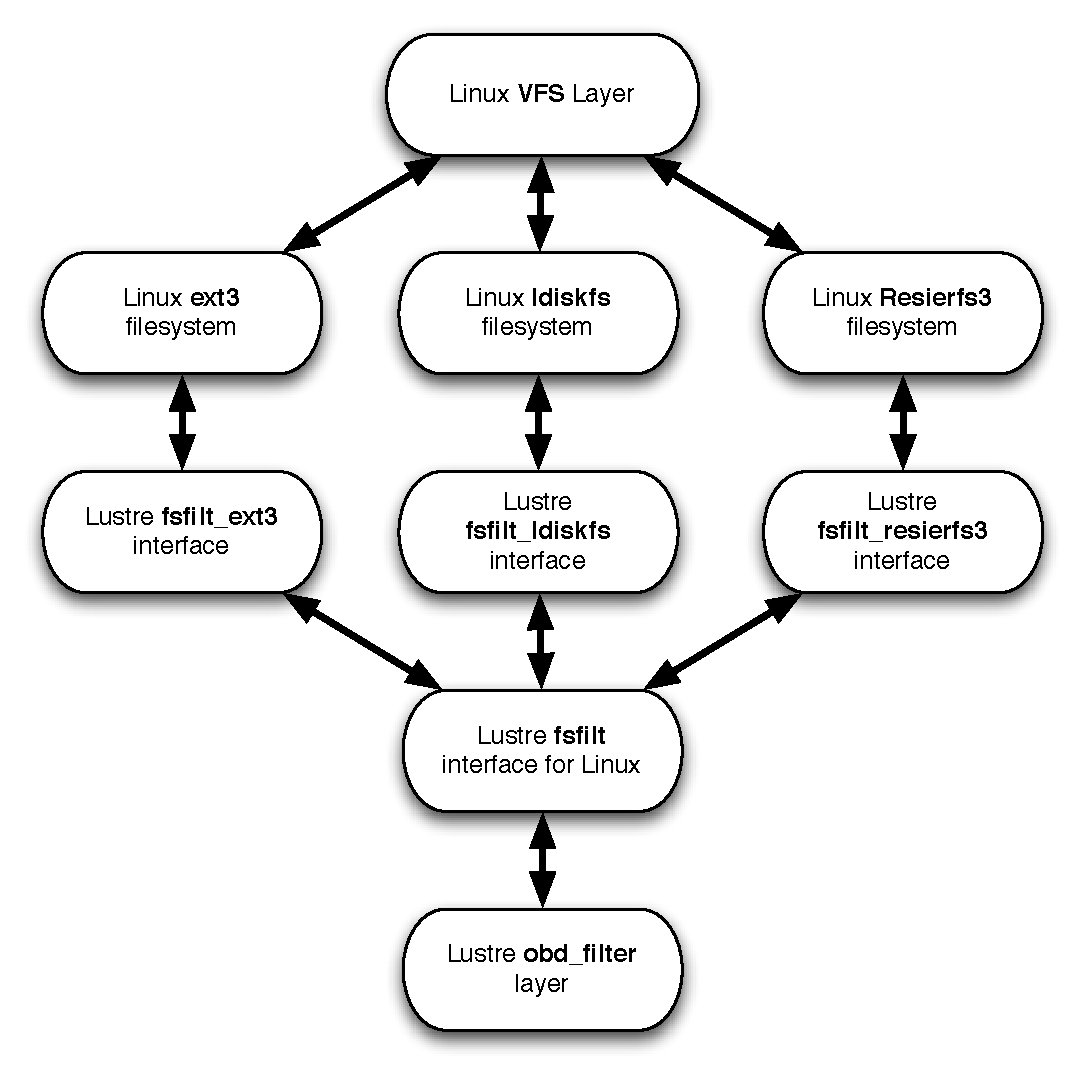
\includegraphics[width=3in]{img/fsfilt_outline}
\caption{An example implementation of the Lustre fsfilt layer.}
\label{fig:fsfilt_outline}
\end{figure}

One interesting point to mention is that although in
the~\url{lustre/lvfs/fsfilt.c} file there are defined symbols
as below:

\begin{Verbatim}
EXPORT_SYMBOL(fsfilt_register_ops);
EXPORT_SYMBOL(fsfilt_unregister_ops);
EXPORT_SYMBOL(fsfilt_get_ops);
EXPORT_SYMBOL(fsfilt_put_ops);
\end{Verbatim}

this file is not used for creating the~\url{fsfilt} kernel module; in fact,
there is no such kernel module. It is linked with \url{lvfs} module to provide
an API to register~\url{fsfilt} methods to access specific filesystems.
The~\url{get_ops} and~\url{put_ops} calls allow those who use~\url{fsfilt}
services to get pointers to appropriate operation tables by names and also to
get a pointer and a reference, so that it is not allowed to
unload the~\url{fsfilt_*} module that is in use. When these functions are stopped
being used, they release respective pointers.

The list below shows~\url{struct fsfilt_operations} methods defined
in the~\url{lustre/include/linux/lustre_fsfilt.h} file.

\begin{Verbatim}
struct fsfilt_operations {
        struct list_head fs_list;
        struct module *fs_owner;
        char   *fs_type;
        char   *(* fs_getlabel)(struct super_block *sb);
        int     (* fs_setlabel)(struct super_block *sb, char *label);
        char   *(* fs_uuid)(struct super_block *sb);
        void   *(* fs_start)(struct inode *inode, int op, void *desc_private,
                             int logs);
        void   *(* fs_brw_start)(int objcount, struct fsfilt_objinfo *fso,
                                 int niocount, struct niobuf_local *nb,
                                 void *desc_private, int logs);
        int     (* fs_extend)(struct inode *inode, unsigned nblocks, void *h);
        int     (* fs_commit)(struct inode *inode, void *handle,int force_sync);
        int     (* fs_commit_async)(struct inode *inode, void *handle,
                                        void **wait_handle);
        int     (* fs_commit_wait)(struct inode *inode, void *handle);
        int     (* fs_setattr)(struct dentry *dentry, void *handle,
                               struct iattr *iattr, int do_trunc);
        int     (* fs_iocontrol)(struct inode *inode, struct file *file,
                                 unsigned int cmd, unsigned long arg);
        int     (* fs_set_md)(struct inode *inode, void *handle, void *md,
                              int size, const char *name);
        int     (* fs_get_md)(struct inode *inode, void *md, int size,
                              const char *name);
        int     (* fs_send_bio)(int rw, struct inode *inode,struct kiobuf *bio);
        ssize_t (* fs_readpage)(struct file *file, char *buf, size_t count,
                                loff_t *offset);
        int     (* fs_add_journal_cb)(struct obd_device *obd, __u64 last_rcvd,
                                      void *handle, fsfilt_cb_t cb_func,
                                      void *cb_data);
        int     (* fs_statfs)(struct super_block *sb, struct obd_statfs *osfs);
        int     (* fs_sync)(struct super_block *sb);
        int     (* fs_map_inode_pages)(struct inode *inode, struct page **page,
                                       int pages, unsigned long *blocks,
                                       int *created, int create,
                                       struct semaphore *sem);
        int     (* fs_write_record)(struct file *, void *, int size, loff_t *,
                                    int force_sync);
        int     (* fs_read_record)(struct file *, void *, int size, loff_t *);
        int     (* fs_setup)(struct super_block *sb);
        int     (* fs_get_op_len)(int, struct fsfilt_objinfo *, int);
        int     (* fs_quotacheck)(struct super_block *sb,
                                  struct obd_quotactl *oqctl);
        __u64   (* fs_get_version) (struct inode *inode);
        __u64   (* fs_set_version) (struct inode *inode, __u64 new_version);
        int     (* fs_quotactl)(struct super_block *sb,
                                struct obd_quotactl *oqctl);
        int     (* fs_quotainfo)(struct lustre_quota_info *lqi, int type,
                                 int cmd);
        int     (* fs_qids)(struct file *file, struct inode *inode, int type,
                            struct list_head *list);
        int     (* fs_get_mblk)(struct super_block *sb, int *count,
                                struct inode *inode, int frags);
        int     (* fs_dquot)(struct lustre_dquot *dquot, int cmd);
        lvfs_sbdev_type (* fs_journal_sbdev)(struct super_block *sb);
};

\end{Verbatim}

\subsection{fsfilt for ext3}
\label{sec:fsfilt_ext3}

As mentioned above, Lustre provides a special~\url{fsfilt} implementation for
every underlying local filesystem. This section explains~\url{fsfilt_ext3}
implementation for the Linux ext3 filesystem. The
~\url{lustre/lvfs/fsfilt_ext3.c} file is used for declaring the~\url{fsfilt}
implementation for ext3. Upon build,~\url{fsfilt_ext3} is plugged into the
kernel as a module. The entry point for the module
is~\url{module_init(fsfilt_ext3_init)} and the exit point
is~\url{module_exit(fsfilt_ext3_exit)}.
 
\begin{Verbatim}
static int __init *fsfilt_ext3_init(void) {}
\end{Verbatim}

is used for initialization at the registration time. All local filesystem
specific~\url{fsfilt} implementations have this call.

Within the \url{init} function, first a cache is created
by~\url{cfs_mem_cache_create()} for the callbacks for journal commits. This
allows a callback to happen when a certain journal transaction is committed.
Currently, Lustre does not support any underlying filesystems without a
journal. The return value for the cache creation in the~\url{init} method is
\url{fcb_cache} variable. Here, \emph{fcb} denotes commit callback data.

Also in the~\url{init} method, the same as any other fsfilt
implementation,~\url{fsfilt_ext3.c} declares the permitted operations for that
particular underlying filesystem by providing a one-to-one mapping between
the~\url{fsfilt} methods and ~\url{fsfilt_ext3} operations through the
~\url{static struct fsfilt_operations fsfilt_ext3_ops={}} definition. Some
important~\url{fsfilt_ext3} methods are explained in more detail below.

\begin{Verbatim}
static void *fsfilt_ext3_start() 
\end{Verbatim}

starts the journal for metadata operations. It checks what kind of operation is
called for through the switch at the beginning of this function call. For each
operation it calculates the maximum number of blocks required for that
particular metadata transaction (denoted by ~\url{nblocks}). For ext3, when a
metadata transaction is initiated, it is required to identify how many blocks
will be used for that transaction. If the requested number of blocks is less than
the available number of blocks, the filesystem will flush some number of blocks
to accommodate the requested block size. This functionality is not required for
a filesystem like ZFS.

\begin{Verbatim}
static char *fsfilt_ext3_get_label()
\end{Verbatim} 

gets the filesystem label, while

\begin{Verbatim}
static char *fsfilt_ext3_set_label()
\end{Verbatim} 

sets the filesystem label.

\begin{Verbatim}
static char *fsfilt_ext3_uuid()
\end{Verbatim}

allows~\url{fsfilt} layer to query the filesystem Linux UUID.

\begin{Verbatim}
static void *fsfilt_ext3_brw_start()
\end{Verbatim} 

starts a journal transaction for the block I/O operation. It takes a buffer of
pages as an argument.

Flow wise, the metadata operations call~\url{*fsfilt_ext3_start()} to open a
journal transaction and do metadata operation, while the block I/O operations
call~\url{*fsfilt_ext3_brw_start()} to open a journal transaction. However,
~\url{*fsfilt_ext3_brw_start()} does not really perform the block I/O but,
rather, generates a journal handle for the transaction. For both operations
the journal is identified by the~\url{*journal} pointer, which is of
type~\url{journal_t}.

Also, as can be seen in the source code, both function calls have
a~\url{*handle} pointer which is of type~\url{handle_t}. This is used for any
operation that requires a journal handle. This handle will be passed as an
argument to its function call.

An important point to mention is that in Lustre when I/O is done to a file,
the inode is modified first and all the required blocks are allocated, then the
transaction is closed and finally the I/O is performed separately, so that the
journal transaction is not kept open for the whole duration of the actual I/O. 

\begin{Verbatim} 
static int fsfilt_ext3_commit() 
\end{Verbatim} 

commits and closes the current open journal transaction. This function also has
a flag called~\url{force_sync}, which signals whether the flush should be
{~\bfseries{\em immediate}}. \url{force_sync=0} means just close the
transaction and {\bfseries{\em do not immediately}} flush, whereas
~\url{force_sync=1} means close the transaction and {\bfseries{\em
immediately}} flush the memory copy.

\begin{Verbatim}
static int fsfilt_ext3_commit_async() 
\end{Verbatim}

also closes the transaction and returns a handle (~\url{**wait_handle}) to
the caller to be used later when actually committing the transaction.

In the true sense of these two operations, \url{fsfilt_ext3_commit} and
\url{fsfilt_ext3_commit_async} are both asynchronous. However with the
availability of the~\url{force_sync} option, the~\url{fsfilt_ext3_commit}
operation has the possibility of synchronously committing a given journal
transaction. Most commonly,~\url{fsfilt_ext3_commit} function is used whereas
~\url{fsfilt_ext3_commit_async} is used exclusively for the~\url{DATA} mode.

\begin{Verbatim}
static int fsfilt_ext3_send_bio()
\end{Verbatim}

submits the I/O to the file. The I/O is already formed before calling this
function such that a list of buffer is created and their destination on the
disk is set in the kernel.  This function is used only for file data, so there
is no need to open a journal transaction at this time. By the time this
function is called, the journal transaction is already closed for performance
reasons. The typical flow for a block I/O is discussed in Section
\ref{sec:fsfilt_examples}. This flow is followed by a
\url{fsfilt_ext3_send_bio} function call for performing the actual block I/O.
For Linux 2.6 kernels all this function does is to call the~\url{submit_bio()}
kernel function. The procedure is more complicated for Linux 2.4 kernels, and it
is beyond the scope of this report.

\begin{Verbatim}
static int fsfilt_ext3_extend()
\end{Verbatim}

extends the journal transaction by the denoted number of blocks. The number of
extra blocks requested is denoted by the~\url{unsigned nblocks}. After the
extension the transaction will still have the same handle denoted by the
~\url{*handle} as Lustre maintains a single transaction visibility. This is
especially useful when it is impossible to predict how many blocks an operation
will take.  Examples where this functionality will be useful are truncate or
unlink operations. 

\begin{Verbatim}
static int fsfilt_ext3_setattr()
\end{Verbatim}

updates the inode size and attributes (user group, access mode, various file
times and file sizes). 

\begin{Verbatim}
static int fsfilt_ext3_iocontrol()
\end{Verbatim}

passes the iocontrol (or ioctl) parameters to the filesystem below.

\begin{Verbatim}
static int fsfilt_ext3_set_md() 
\end{Verbatim}

and

\begin{Verbatim}
static int fsfilt_ext3_get_md()
\end{Verbatim}


are used for setting and querying the striping information. For ext3 this
information is kept in EA, and the implementation is filesystem specific.

\begin{Verbatim}
static size_t fsfilt_ext3_readpage()
\end{Verbatim}

is for reading a page from the underlying file or directory. The switch at the
begining of this function determines if it is a file or a directory to be
read. If it is a normal file, then it simply calls a~\url{read()} kernel
function to fill in the buffer with the file data information. However, if it is a
directory to be read, then it calls ext3 directory read functions to read from
the directory. 

\begin{Verbatim}
static int fsfilt_ext3_add_journal_cb()
\end{Verbatim}

is used for updating the in-memory representation of what is actually committed
on disk on a server from a transaction point of view. This is useful when
replying to a client with the in-memory representation of what is actually
committed on disk on that particular server for that particular client, so that
the client can discard all data up to that given transaction number to save
memory. The advantage of having this functionality is that, in case of a server
crash, the data will still be in the client's memory since the server wouldn't have
responded back with the~\url{*cb_data} yet. Here,~\url{*cb_data} holds the
pointer address for the number of the last committed transaction on the disk. The drawback
is that by keeping an extra copy on the client (besides the copy on the server), memory consumption is increased.

\begin{Verbatim}
int fsfilt_ext3_map_ext_inode_pages()
\end{Verbatim}

is the function that allocates the blocks. It is used to get
information about blocks underlying a certain block range and if they are not
allocated, then it allocates them if requested. It sends the requestor an array of
pages where the blocks are placed. 

\begin{Verbatim}
static int fsfilt_ext3_write_record()
\end{Verbatim}

and

\begin{Verbatim}
static int fsfilt_ext3_read_record()
\end{Verbatim}

are for journal update of the special~\url{LLOG} (Lustre Log) file. This file
is automatically updated. The~\url{LLOG} is required while performing an operation
on multiple nodes (e.g., unlink, which has to start on the MDS and then continue
on the OSTs). 

\begin{Verbatim}
static int fsfilt_ext3_setup()
\end{Verbatim}

is used when the ext3 filesystem is first mounted. The~\url{obd_filter}
initialization calls this function.

\begin{Verbatim}
static int fsfilt_ext3_get_op_len()
\end{Verbatim}

is to get the number of blocks in the journal that a particular operation will
require. This function is obsolete and not called at all.

\begin{Verbatim}
static __u64 fsfilt_ext3_get_version()
\end{Verbatim}

and

\begin{Verbatim}
static __u64 fsfilt_ext3_set_version()
\end{Verbatim}

are for setting and querying the inode version. Inode version is currently not
used in the code base we have discussed so far. However, in future code bases,
it will be used for version based recovery mechanisms.

\subsection{fsfilt Use Case Examples}
\label{sec:fsfilt_examples}

Typical flows for metadata operations, asynchronous block I/O operations, and
synchronous block I/O operations can be seen in Figures
~\ref{fig:fsfilt_metadata}, \ref{fig:fsfilt_data_async}, and
\ref{fig:fsfilt_data_sync}, respectively.

Figure~\ref{fig:fsfilt_metadata} is an example of a metadata operation. This
type of flow is used in Lustre either when there is no file data or when no
client is available for replying to a certain set of metadata operations.

\begin{figure}[hbt]
\centering
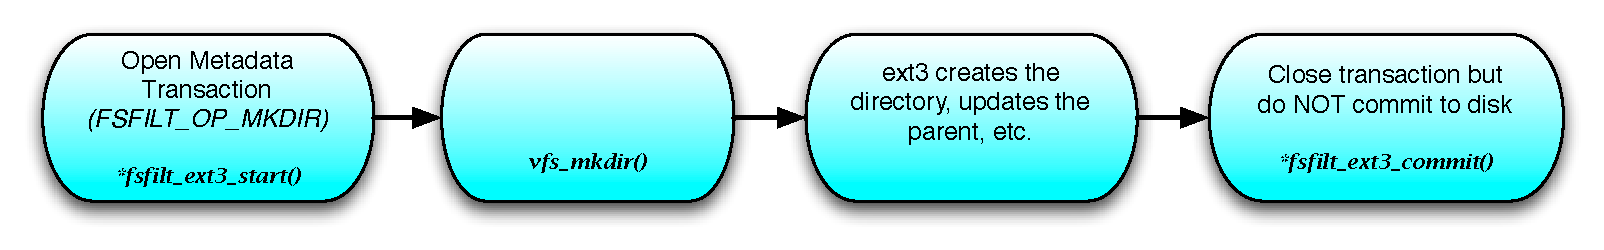
\includegraphics[width=4.5in]{img/fsfilt_metadata}
\caption{Fsfilt flow path for metadata operations.}
\label{fig:fsfilt_metadata}
\end{figure}

\begin{figure}[hbt]
\centering
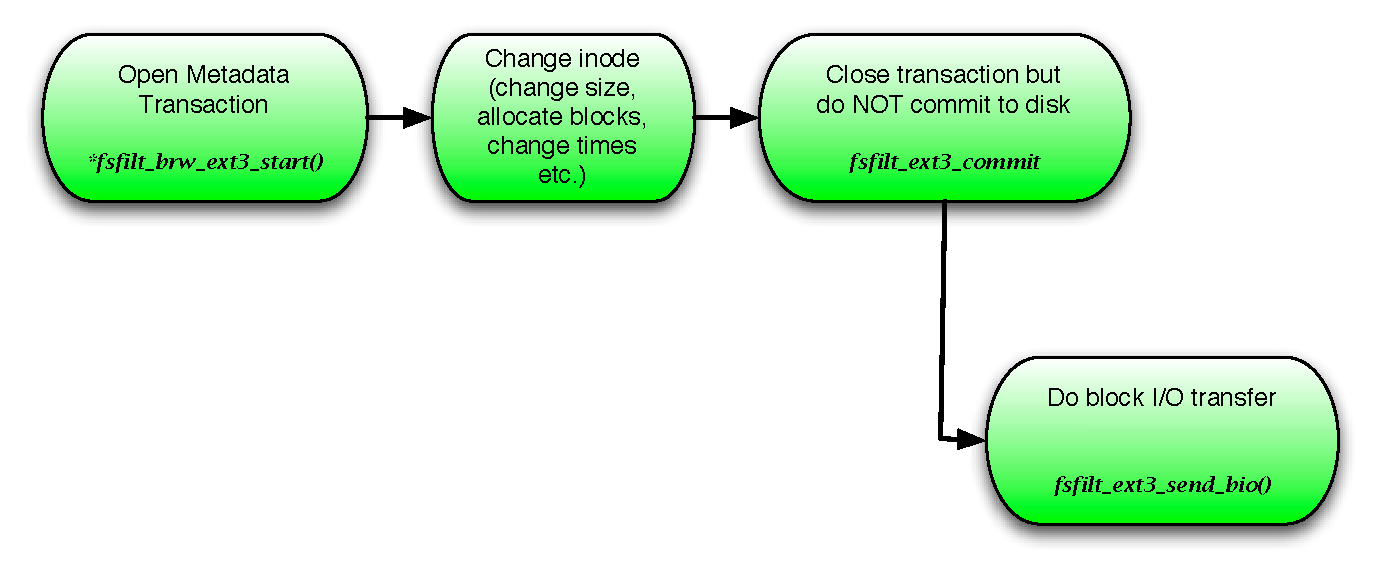
\includegraphics[width=5in]{img/fsfilt_data_async}
\caption{Fsfilt flow path for asynchronous block I/O operations.}
\label{fig:fsfilt_data_async}
\end{figure}

\begin{figure}[hbt]
\centering
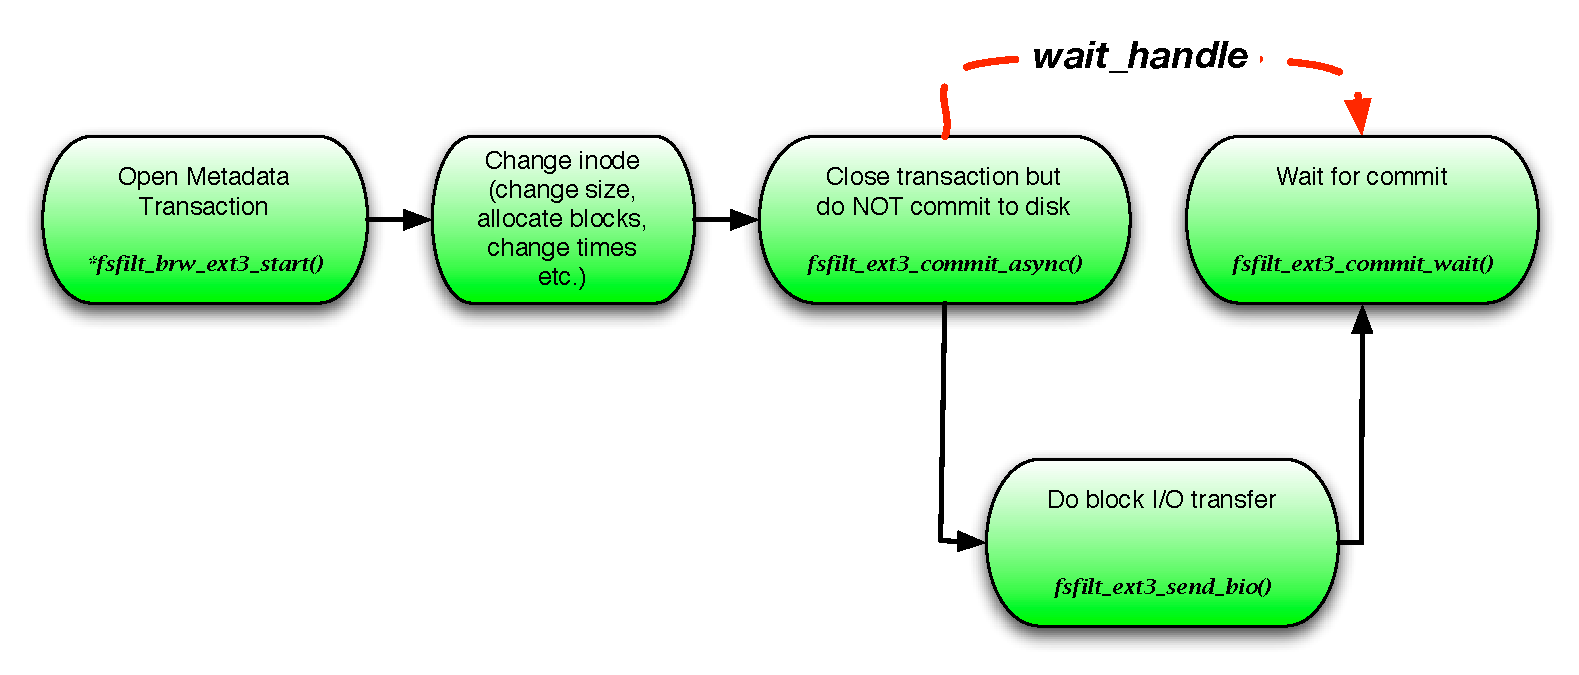
\includegraphics[width=5in]{img/fsfilt_data_sync}
\caption{Fsfilt flow path for synchronous block I/O operations.}
\label{fig:fsfilt_data_sync}
\end{figure}

\subsubsection{\texttt{\small DIRECT\_IO} in Lustre}

Lustre uses~\url{DIRECT_IO} for all file data I/O operations from
the~\url{obd_filter} to disk and back (not cached at any point). The metadata
is always journaled.

As can be seen from Figures~\ref{fig:fsfilt_data_async}
and~\ref{fig:fsfilt_data_sync}, these flows guarantee that the data is actually
written to the disk before the journal transaction is committed. These flows
represent the~\url{ORDERED} journal mode with~\url{DIRECT_IO}. In the~\url{DATA}
mode, the bulk data is written to the journal first and then after it is
committed to the journal, file data is transferred to the disk.

\subsubsection{Replaying Last Transactions After a Server Crash}

As an example, let's consider the following. Client connects and performs some
operations on a Lustre server. Server replies back to the client with a commit,
but at this point the data is actually not committed to the disk.  Client now
has the record of the last transaction being committed as $ x+y $ while 
according to the server disk, it is just $ x $. If the server crashes at this
point, there is a conflict between the server disk and client in terms of the
last committed transaction number. Let's further assume that following this chain of
events, the server is rebooted and the client reconnects to the server. The
server then replies back with acknowledgment and the number of the last
transaction from that client that is already committed to the server disk. For
our example this number is $ x $. The client then replies back with $ x + 5 $
being the last transaction number committed by that server and a list of the five last
missing transactions to be performed by the server.

\subsubsection{Client Connect/Disconnect}

Another use case example for ~\url{fsfilt_ext3_commit} with ~\url{force_sync = 1} in
Lustre would be the client connect/disconnect case. Each Lustre server
maintains a separate table of client connect/disconnect operations. This table
is kept on a separate file on each server and is journaled.  When a client
connects, it is written to a separate file and this file is fully journaled. To
maintain this file,~\url{fsfilt_ext3_commit} is used and the~\url{force_sync}
flag is set to 1, as there would be no client to reply after a replay if the
client is already disconnected.

\subsubsection{Why \texttt{\small ls} Is Expensive on Lustre}

As an example let's consider the~\url{ls} operation on an ext3 based Lustre
filesystem which is actually performed using the~\url{fsfilt_ext3_readpage}
behind the scenes.  From the client perspective, it connects to the MDS and gets
the content and inode number for that particular directory it is interested in.
Based on the content information, the client then sends~\url{stats} requests
for each file in that directory back to the MDS. The MDS will reply back with
striping information for each stat request (as well as with other pertinent
file metadata per request). All of these are completed in separate RPCs. If,
for example, there are three files in that given directory, by the end of this
step, the client would have sent five separate RPCs to the MDS (dir open, readdir,
and stats for every file). (In fact, regular~\url{ls} does not need the file
mode during~\url{ls}, but most Linux distributions are now delivered with
``color ls" that wants to output file information in color depending on file
type, so it does a~\url{stat()} call for every file.)  Following this step, if
the client is interested in file size data, as an example, it has to query all the
OSTs that were listed in the stat information by sending glimpse RPCs. This step
has to be repeated for every file separately. Again, as an example, if each of
those three files are striped over 100 OSTs, by the end of this step, client would
have sent $ 3 + ( 3 \times 100) $, or in other words, 305 RPCs. This is true
not only for the~\url{ls -l} but also for the regular~\url{ls} case,
such that it needs to find the file mode.
